% Options for packages loaded elsewhere
\PassOptionsToPackage{unicode}{hyperref}
\PassOptionsToPackage{hyphens}{url}
%
\documentclass[
  ignorenonframetext,
  aspectratio=169]{beamer}
\usepackage{pgfpages}
\setbeamertemplate{caption}[numbered]
\setbeamertemplate{caption label separator}{: }
\setbeamercolor{caption name}{fg=normal text.fg}
\beamertemplatenavigationsymbolsempty
% Prevent slide breaks in the middle of a paragraph
\widowpenalties 1 10000
\raggedbottom
\setbeamertemplate{part page}{
  \centering
  \begin{beamercolorbox}[sep=16pt,center]{part title}
    \usebeamerfont{part title}\insertpart\par
  \end{beamercolorbox}
}
\setbeamertemplate{section page}{
  \centering
  \begin{beamercolorbox}[sep=12pt,center]{part title}
    \usebeamerfont{section title}\insertsection\par
  \end{beamercolorbox}
}
\setbeamertemplate{subsection page}{
  \centering
  \begin{beamercolorbox}[sep=8pt,center]{part title}
    \usebeamerfont{subsection title}\insertsubsection\par
  \end{beamercolorbox}
}
\AtBeginPart{
  \frame{\partpage}
}
\AtBeginSection{
  \ifbibliography
  \else
    \frame{\sectionpage}
  \fi
}
\AtBeginSubsection{
  \frame{\subsectionpage}
}
\usepackage{lmodern}
\usepackage{amssymb,amsmath}
\usepackage{ifxetex,ifluatex}
\ifnum 0\ifxetex 1\fi\ifluatex 1\fi=0 % if pdftex
  \usepackage[T1]{fontenc}
  \usepackage[utf8]{inputenc}
  \usepackage{textcomp} % provide euro and other symbols
\else % if luatex or xetex
  \usepackage{unicode-math}
  \defaultfontfeatures{Scale=MatchLowercase}
  \defaultfontfeatures[\rmfamily]{Ligatures=TeX,Scale=1}
\fi
% Use upquote if available, for straight quotes in verbatim environments
\IfFileExists{upquote.sty}{\usepackage{upquote}}{}
\IfFileExists{microtype.sty}{% use microtype if available
  \usepackage[]{microtype}
  \UseMicrotypeSet[protrusion]{basicmath} % disable protrusion for tt fonts
}{}
\makeatletter
\@ifundefined{KOMAClassName}{% if non-KOMA class
  \IfFileExists{parskip.sty}{%
    \usepackage{parskip}
  }{% else
    \setlength{\parindent}{0pt}
    \setlength{\parskip}{6pt plus 2pt minus 1pt}}
}{% if KOMA class
  \KOMAoptions{parskip=half}}
\makeatother
\usepackage{xcolor}
\IfFileExists{xurl.sty}{\usepackage{xurl}}{} % add URL line breaks if available
\IfFileExists{bookmark.sty}{\usepackage{bookmark}}{\usepackage{hyperref}}
\hypersetup{
  pdftitle={Wow! The beauty of friesland},
  pdfauthor={Jannick Akkermans (1727324)},
  hidelinks,
  pdfcreator={LaTeX via pandoc}}
\urlstyle{same} % disable monospaced font for URLs
\newif\ifbibliography
\usepackage{graphicx,grffile}
\makeatletter
\def\maxwidth{\ifdim\Gin@nat@width>\linewidth\linewidth\else\Gin@nat@width\fi}
\def\maxheight{\ifdim\Gin@nat@height>\textheight\textheight\else\Gin@nat@height\fi}
\makeatother
% Scale images if necessary, so that they will not overflow the page
% margins by default, and it is still possible to overwrite the defaults
% using explicit options in \includegraphics[width, height, ...]{}
\setkeys{Gin}{width=\maxwidth,height=\maxheight,keepaspectratio}
% Set default figure placement to htbp
\makeatletter
\def\fps@figure{htbp}
\makeatother
\setlength{\emergencystretch}{3em} % prevent overfull lines
\providecommand{\tightlist}{%
  \setlength{\itemsep}{0pt}\setlength{\parskip}{0pt}}
\setcounter{secnumdepth}{-\maxdimen} % remove section numbering

\title{Wow! The beauty of friesland}
\author{Jannick Akkermans (1727324)}
\date{24-11-2021}

\begin{document}
\frame{\titlepage}

\begin{frame}{Overview}
\protect\hypertarget{overview}{}

\begin{itemize}
  \item The flag of Friesland
  \item The province of Friesland
  \item General feeling of unsafety in Friesland
  \item Population statistics of Friesland
  \item Pros and cons of Friesland
  \item Estimation of population growth
\end{itemize}

\end{frame}

\begin{frame}{The flag of Friesland}
\protect\hypertarget{the-flag-of-friesland}{}

\begin{figure}
  \center
  \includegraphics[width=80mm]{"Flag-of-Friesland.png"}
  \caption{The beautiful flag of Friesland}
\end{figure}

\end{frame}

\begin{frame}[fragile]{General feeling of unsafety in Friesland}
\protect\hypertarget{general-feeling-of-unsafety-in-friesland}{}

\begin{verbatim}
## Loading required package: plotly
\end{verbatim}

\begin{verbatim}
## Warning: package 'plotly' was built under R version 4.1.2
\end{verbatim}

\begin{verbatim}
## 
## Attaching package: 'plotly'
\end{verbatim}

\begin{verbatim}
## The following object is masked from 'package:ggplot2':
## 
##     last_plot
\end{verbatim}

\begin{verbatim}
## The following object is masked from 'package:stats':
## 
##     filter
\end{verbatim}

\begin{verbatim}
## The following object is masked from 'package:graphics':
## 
##     layout
\end{verbatim}

\begin{verbatim}
## Loading required package: scales
\end{verbatim}

\begin{verbatim}
## 
## Attaching package: 'scales'
\end{verbatim}

\begin{verbatim}
## The following object is masked from 'package:purrr':
## 
##     discard
\end{verbatim}

\begin{verbatim}
## The following object is masked from 'package:readr':
## 
##     col_factor
\end{verbatim}

\end{frame}

\begin{frame}{Slide with Plot}
\protect\hypertarget{slide-with-plot}{}

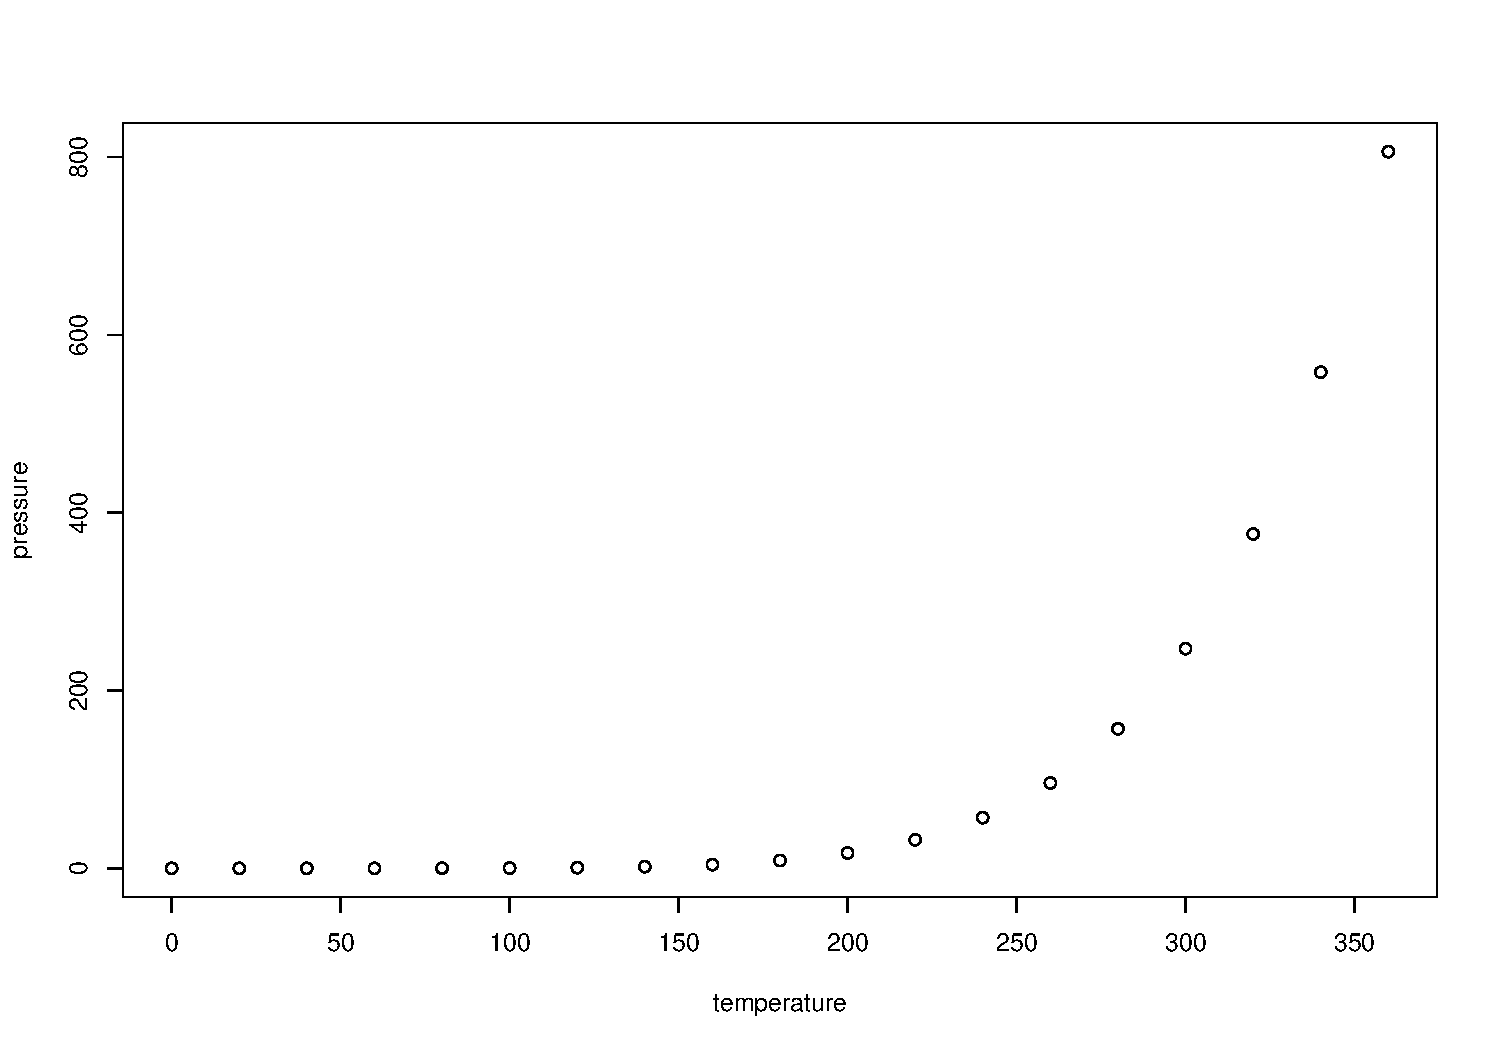
\includegraphics{friesland_files/figure-beamer/pressure-1.pdf}

\end{frame}

\end{document}
